\documentclass[conference]{IEEEtran}

\usepackage{cite}
\usepackage{amsmath,amssymb}
\usepackage{booktabs}
\usepackage{array}
\usepackage{tabularx}
\usepackage{url}
\usepackage{graphicx}
\usepackage{float}
\usepackage{placeins}

\setlength{\textfloatsep}{4pt plus 1.0pt minus 1.0pt}
\setlength{\floatsep}{3pt plus 1.0pt minus 1.0pt}
\setlength{\intextsep}{3pt plus 1.0pt minus 1.0pt}
\setlength{\abovecaptionskip}{2pt}
\setlength{\belowcaptionskip}{2pt}

\title{Phoenix: Deterministic Self-Healing and Fault Tolerance for Autonomous Desktop Automation}

\author{
\IEEEauthorblockN{
Ramani G\textsuperscript{1},
Akshitha V G\textsuperscript{2},
Kruthin Shanmuk Yadav CG\textsuperscript{3},
Dhanyashree G V\textsuperscript{4},
Kaushal K\textsuperscript{5}
}
\IEEEauthorblockA{
Department of Computer Science and Engineering (AI \& ML)\\
AMC Engineering College, Bengaluru, Karnataka, India\\
Emails: gowrisan.ramani@amceducation.in, akshithavg1@gmail.com, \\
kruthin008@gmail.com, dhanyashreegv206@gmail.com, kaushalk123000@gmail.com
}
}

\begin{document}

\maketitle

\begin{abstract}
Reliable execution in multi-agent desktop automation requires robust error mitigation beyond raw task scheduling. Real-world automation workflows routinely encounter application crashes, missing file dependencies, transient network timeouts, and unauthorized operations. Existing AI agent recovery approaches rely heavily on continuous model-based replanning, which can introduce inference latency, token usage, and behavioral variability. In this paper, we present the self-healing subsystem of Phoenix Agents, a deterministic, bounded recovery framework designed to diagnose and remediate execution exceptions in multi-agent desktop workflows without requiring an active Large Language Model (LLM) during the recovery loop. The recovery mechanism is structured into five operational stages: error parsing, root-cause classification, strategy selection, patch generation, and retry execution. Recovery decisions follow typed contract assertions, deterministic rules, and a fixed retry budget ($K_{\text{max}} = 3$). Empirical evaluation across 125 controlled fault-injection trials (25 per class across five fault categories) demonstrates that the pipeline achieved a 66.7\% recovery rate (50/75, Wilson 95\% CI: [55.4\%, 76.3\%]) across the 75 recoverable-by-design faults (recovering 25/25 Timeout and 25/25 Missing Resource, while Tool/Adapter faults were rejected as unmapped), and safely rejected all 50 non-recoverable faults (100.0\%, Wilson 95\% CI: [92.9\%, 100.0\%], $n=50$) across Permission/Policy Violation and Unmapped/Unknown Exception. Overall recovery across all 125 faults was 40.0\% (50/125, Wilson 95\% CI: [31.8\%, 48.8\%]), with an 80.0\% total correct decision rate (100/125, Wilson 95\% CI: [72.1\%, 86.1\%]), compared to 20.0\% (25/125) for naive retry and 0.0\% (0/125) for fail-fast. Mean recovery latency was 2.06~ms (median 1.98~ms) on mocked adapters and 2.30~ms for real-filesystem missing resource synthesis.
\end{abstract}

\begin{IEEEkeywords}
Phoenix Agents, Self-Healing, Multi-Agent Systems, Desktop Automation, Fault Recovery, Deterministic Recovery, Error Mitigation.
\end{IEEEkeywords}

\section{Introduction}
Multi-agent desktop and browser automation frameworks orchestrate complex workflows across web browsers, native applications, operating system terminals, and local file systems~\cite{bajoria2026}. However, executing tasks across heterogeneous host environments inherently exposes software agents to dynamic execution failures, such as transient network timeouts, missing file dependencies, altered DOM locators, process crashes, and permission denials.

In conventional script-based automation systems (e.g., Selenium, AutoHotkey), a single runtime exception causes catastrophic workflow failure. While recent research explores self-healing via Large Language Models (LLMs)---such as reflective prompt loops and continuous model replanning---each LLM call in recovery incurs latency and token cost that depend on the model and prompt size, along with safety risks from uncontrolled retries~\cite{babu2026,jeong2026}.

To address these challenges, we present the deterministic self-healing architecture of Phoenix Agents. Phoenix Agents uses an in-process asynchronous publish--subscribe EventBus for event delivery, while the five recovery stages execute sequentially within the recovery handler. The framework uses a lightweight 5-stage pipeline (Error Parsing, Root-Cause Analysis, Strategy Selection, Patch Generation, and Retry Execution) that diagnoses and remediates execution errors without requiring an active LLM runtime during error recovery.

The Primary Technical Contributions of This Paper:
\begin{itemize}
    \item \textbf{Structured 5-Stage Self-Healing Pipeline:} A modular recovery architecture executing error parsing, root-cause diagnosis, strategy selection, patch generation, and retry dispatch without LLM inferencing delays.
    \item \textbf{Deterministic In-Process Recovery Loop:} Rule-based mitigation policies and typed contract assertions achieving millisecond-scale handling latency (mean $T_R = 2.05$~ms, $T_{\text{rec}} = 2.06$~ms on mocked adapters; 2.30~ms on real filesystem).
    \item \textbf{Bounded Retry \& Safety Guard Policy:} Strict enforcement of a maximum retry limit ($K_{\text{max}} = 3$) paired with safe rejection of non-recoverable operations (100.0\% safe rejection over 50 non-recoverable faults, Wilson 95\% CI: [92.9\%, 100.0\%], $n=50$).
    \item \textbf{Empirical Verification Across 125 Controlled Trials:} Controlled fault-injection evaluation across 125 trials (25 per class across five classes), reporting both the aggregate recovery rate (40.0\%, 50/125, Wilson 95\% CI: [31.8\%, 48.8\%]; 80.0\% correct decision rate, 100/125) and the recoverable subset rate (66.7\%, 50/75, Wilson 95\% CI: [55.4\%, 76.3\%]) side-by-side, establishing clear differentiation against naive retry (20.0\% overall recovery; 0.0\% safe rejection).
\end{itemize}

\section{Related Work}

\subsection{Self-Healing Agent Orchestrators and LLM Recovery}
Recent studies explore self-healing mechanisms to improve the operational reliability of tool-augmented Large Language Model (LLM) agents. Babu and Agrawal proposed self-healing orchestrators for LLM tool agents, emphasizing reflective prompt loops for fault correction~\cite{babu2026}. Jeong and Shin investigated autonomous self-healing frameworks for LLM agents~\cite{jeong2026}. Patel et al.\ explored predictive self-healing using Model Predictive Control (MPC)~\cite{patel2026a} and multi-agent learning~\cite{patel2026b}. While these approaches improve adaptability, invoking generative models during error recovery inherently incurs latency and token cost that depend on the underlying model and prompt size, alongside potential variability in recovery decisions.

\subsection{Fault-Tolerant Multi-Agent Collaboration}
In multi-agent systems, fault tolerance research addresses role drift, agent disagreements, and dynamic environment reconfigurations. Wang et al.\ developed lightweight protocols to detect and repair role drift in collaborative multi-agent workflows~\cite{wang2026}. Ju et al.\ investigated self-repair capabilities elicited under LLM multi-agent disagreements~\cite{ju2025}. Guo et al.\ introduced EvoConfig for self-evolving multi-agent configuration~\cite{guo2026}. Bara et al.\ demonstrated self-healing multi-agent pipelines for machine learning workflows~\cite{bara2026}. Phoenix Agents complements this line of research by addressing discrete workflow execution exceptions through structured fault taxonomies and bounded deterministic rules.

\subsection{Web and GUI Automation Reliability}
In web and desktop automation, fault recovery historically focused on dynamic locator repair and selector maintenance during UI test execution~\cite{garcia2026}. Surveys by Nguyen et al.~\cite{nguyen2025} and Bajoria et al.~\cite{bajoria2026} highlight that GUI agents frequently fail due to unhandled ambient operating system noise, dynamic DOM updates, and transient network delays. Traditional GUI testing frameworks lack dependency-aware task graphs and supervisory contracts required for autonomous, multi-application workflow recovery.

\subsection{Research Gap \& Key Differentiation}
Existing self-healing literature focuses primarily on model-driven reflection or continuous replanning~\cite{babu2026,jeong2026,patel2026a}. These approaches often rely on generative replanning where each LLM invocation adds model-dependent latency and cost, and they frequently lack strict safety guards, resulting in uncontrolled retries of unsafe system operations. Phoenix Agents bridges this gap by decoupling error diagnosis from LLM runtime inferencing, executing a 5-stage bounded recovery pipeline sequentially within the recovery handler to achieve millisecond-scale recovery latency (mean $T_R = 2.05$~ms, $T_{\text{rec}} = 2.06$~ms) alongside 100.0\% safe rejection of non-recoverable operations.

\section{Proposed Solution: 5-Stage Deterministic Self-Healing Architecture}
The proposed self-healing subsystem of Phoenix Agents is designed as an in-process, deterministic recovery framework that remediates execution exceptions without invoking active LLM inference during the recovery loop. Normal workflow dispatch and fault handling are kept as decoupled, specialized subsystems communicating asynchronously over the publish--subscribe EventBus.

\subsection{Formal Problem Formulation \& Recovery Objectives}
Let a workflow execution graph be represented as a Directed Acyclic Graph $G = (V, E)$. When the Supervisor Agent audits post-execution task outputs $O_i$ against contract assertions $\Psi(v_i, O_i)$, any failure triggers an observed execution fault tuple:
\begin{equation}
F = (E_{\text{err}}, C_{\text{ctx}}, S_{\text{workflow}})
\end{equation}
where $E_{\text{err}}$ represents the captured exception traceback, $C_{\text{ctx}}$ represents execution parameters and tool adapter state, and $S_{\text{workflow}}$ is the atomic graph lifecycle state.

\begin{figure}[!t]
    \centering
    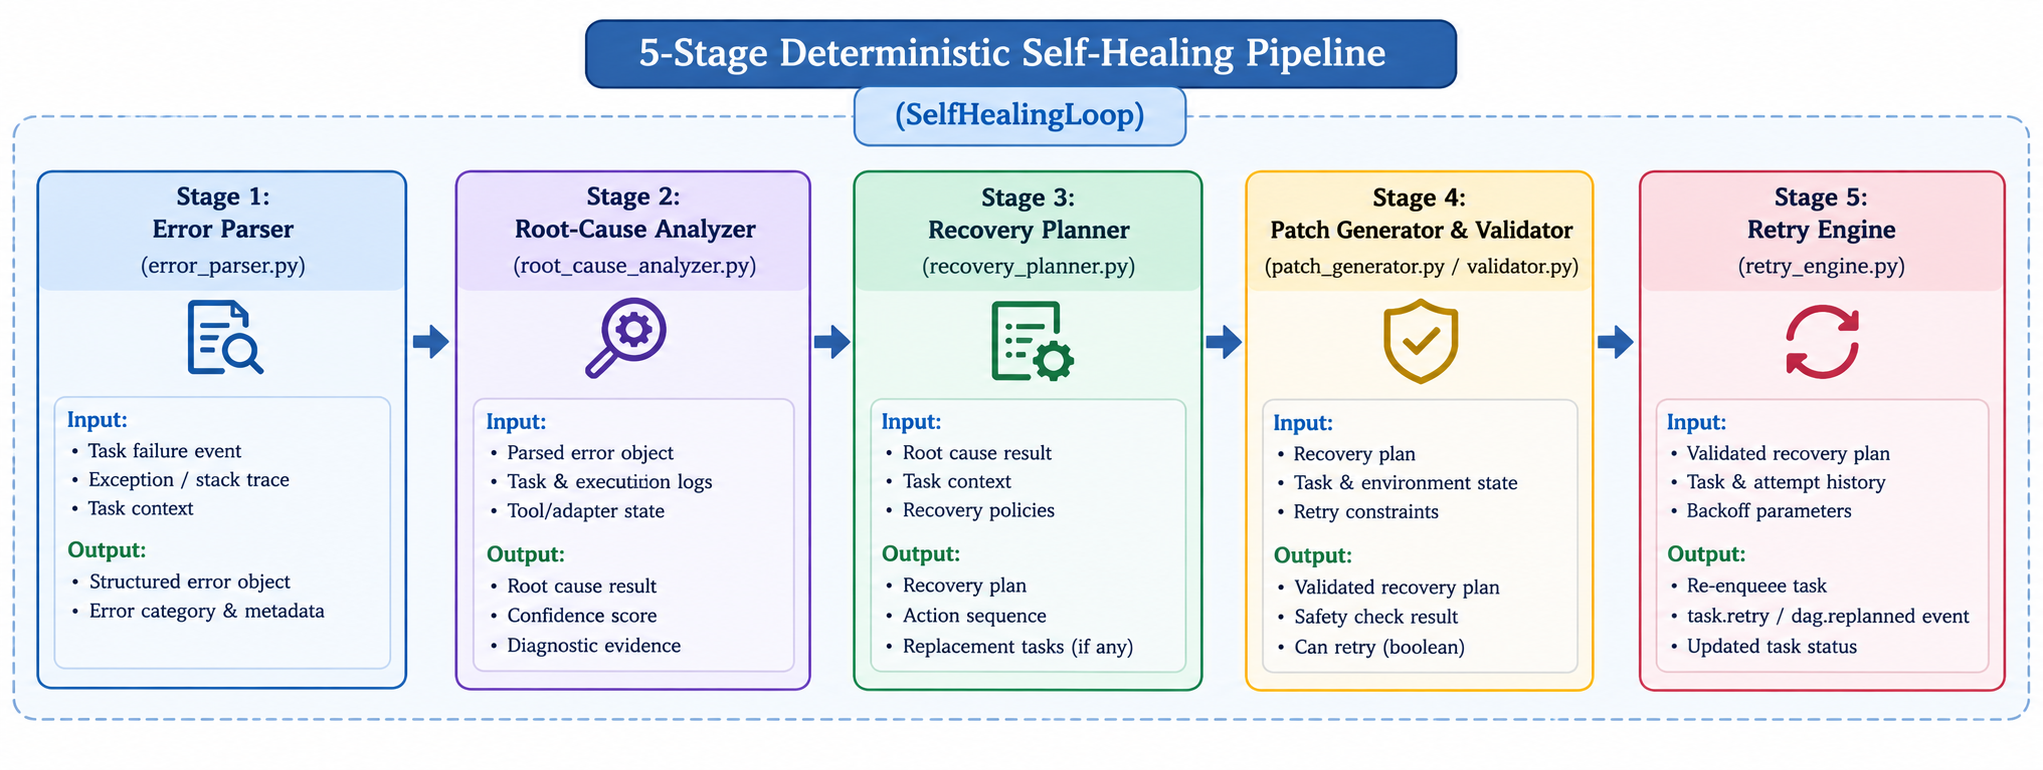
\includegraphics[width=0.95\columnwidth]{extracted_figures/fig_p2__Im1.png}
    \caption{Five-stage deterministic self-healing architecture of Phoenix Agents.}
    \label{fig:architecture}
\end{figure}

The recovery objective function $R(F)$ maps observed faults to either permitted remediation actions or safe terminal rejections:
\begin{equation}
R(F) =
\begin{cases}
A_{\text{retry}}, & \text{if } F \in \mathcal{C}_{\text{recoverable}} \land k_i < K_{\text{max}}, \\
A_{\text{reject}}, & \text{if } F \in \mathcal{C}_{\text{nonrec}} \lor k_i \ge K_{\text{max}}.
\end{cases}
\end{equation}
where $k_i$ is the retry counter for task $v_i$, $K_{\text{max}} = 3$ is the maximum allowed retry budget, $A_{\text{retry}}$ applies deterministic parameter patching or backoff retry, and $A_{\text{reject}}$ triggers safe failure escalation.

\subsection{Detailed 5-Stage Recovery Pipeline Breakdown}
The self-healing workflow is executed sequentially across five specialized, in-process software modules:

\subsubsection{Stage 1: Error Parser (\texttt{error\_parser.py})}
Intercepts published \texttt{task.failed} event payloads and parses unhandled stack traces into structured error objects, extracting error strings, failing module paths, adapter bindings $\tau_i$, and payload parameters $\theta_i$.

\subsubsection{Stage 2: Root-Cause Analyzer (\texttt{root\_cause\_analyzer.py})}
Evaluates parsed error objects against deterministic rule sets to classify faults into a 5-tier taxonomy:
\begin{equation}
\mathcal{C} \in
\begin{Bmatrix}
\text{Timeout}, \quad \text{Missing Resource}, \\
\text{Tool/Adapter Failure}, \\
\text{Permission/Policy Violation}, \\
\text{Unmapped/Unknown Exception}
\end{Bmatrix}
\end{equation}

\subsubsection{Stage 3: Recovery Planner (\texttt{recovery\_planner.py})}
Evaluates whether the classified fault is recoverable and checks retry budget constraints ($k_i < K_{\text{max}}$). If $k_i \ge K_{\text{max}}$ or if the fault is classified as non-recoverable (Permission/Policy Violation, Unmapped/Unknown Exception), it marks the task as unrecoverable and emits a \texttt{task.rejected} event.

\subsubsection{Stage 4: Patch Generator (\texttt{patch\_generator.py})}
Constructs the required corrective action using the selected deterministic recovery strategy:
\begin{itemize}
    \item \textbf{Exponential Backoff:} Calculates delay $\Delta t = 2^{k_i} \times 1.0\,\text{s}$ for Timeout faults.
    \item \textbf{Parameter Patching:} Corrects missing file paths or parameters in $\theta_i$ by inspecting ancestor task outputs in graph $G$ or synthesizing target resource paths.
    \item \textbf{Adapter Substitution:} Queries \texttt{ToolRegistry} for a functional substitute adapter $\tau'_i$ for Tool/Adapter Failure faults.
\end{itemize}

\subsubsection{Stage 5: Retry Engine (\texttt{retry\_engine.py})}
Applies generated patches, increments retry counter $k_i \leftarrow k_i + 1$, resets task status $S_i \leftarrow \text{READY}$, and dispatches a typed \texttt{task.retry} event over the EventBus.

\section{Methodology and Implementation}
The self-healing architecture of Phoenix Agents is implemented as a modular Python package integrated directly within the execution engine kernel.

\subsection{Asynchronous In-Process Event Backbone (EventBus)}
Phoenix Agents uses an in-process asynchronous publish--subscribe EventBus for event delivery, while the five recovery stages execute sequentially within the recovery handler. The EventBus is constructed over Python's native \texttt{asyncio} event loop. Rather than incurring network IPC delays, event objects are published directly to memory channels.

When a tool adapter fails, the Worker Agent publishes a strongly typed \texttt{task.failed} event containing:
\begin{equation}
\text{Payload} = \langle \text{task\_id}, \tau_i, \theta_i, e_{\text{exception}}, \text{traceback\_str} \rangle
\end{equation}
Handler callbacks in the Healing Agent process events asynchronously as non-blocking coroutines without stalling concurrent DAG task branches.

\subsection{Supervisory Contract Verification Engine (SupervisorAgent)}
Before a task is marked as completed, the Supervisor Agent evaluates tool execution artifacts $O_i$ against pre-registered contract assertions:
\begin{align}
\Psi(v_i, O_i) = (\text{exit\_code} == 0) &\land (O_i \models \text{Schema}(v_i)) \nonumber \\
&\land (\text{FileExists}(O_i))
\end{align}
If any assertion evaluates to false, the Supervisor transitions the node status $S_i \leftarrow \text{FAILED}$ and publishes the failure diagnostic payload to trigger self-healing.

\subsection{Fault Taxonomy \& Pattern Matching Classifier (\texttt{root\_cause\_analyzer.py})}
The Root-Cause Analyzer processes exception strings using deterministic rule matching across a 5-tier taxonomy: recoverable faults comprise \textit{Timeout} (mitigated via bounded retry with exponential backoff), \textit{Missing Resource} (parameter/path correction from ancestor task outputs or directory creation), and \textit{Tool/Adapter Failure} (intended for adapter substitution via \texttt{ToolRegistry}); non-recoverable faults comprise \textit{Permission/Policy Violation} and \textit{Unmapped/Unknown Exception}, both mapped to immediate safe rejection and failure escalation.

\subsection{Parameter Patching \& Adapter Resolution (\texttt{patch\_generator.py})}
\begin{itemize}
    \item \textbf{Parameter Patching:} For Missing Resource faults, the Patch Generator inspects ancestor node output dictionaries in graph $G$ to resolve valid target file paths or synthesizes missing directory trees within workspace boundaries.
    \item \textbf{Adapter Substitution:} For Tool/Adapter Failure faults, the component queries \texttt{ToolRegistry} to resolve a functional substitute adapter $\tau'_i$. In our evaluated 125-fault benchmark suite, injected tool failures used unmapped command error strings that were classified as unknown and safely rejected; adapter substitution was evaluated in separate component unit tests.
\end{itemize}

\section{Empirical Evaluation \& Experimental Results}

\subsection{Experimental Setup}
All experiments were conducted on a workstation equipped with an AMD Ryzen 7 8845HS processor (16 logical execution threads), 15.26~GB RAM, running Windows 11 Home (build 10.0.26300) and Python 3.14.4. 

The evaluation suite comprised 125 controlled fault injections (25 distinct faults per class across five classes):
\begin{enumerate}
    \item \textit{Timeout} (25 faults, recoverable by design);
    \item \textit{Missing Resource} (25 faults, recoverable by design);
    \item \textit{Tool/Adapter Failure} (25 faults, recoverable by design);
    \item \textit{Permission/Policy Violation} (25 faults, non-recoverable);
    \item \textit{Unmapped/Unknown Exception} (25 faults, non-recoverable).
\end{enumerate}
The test workloads comprised 3--5 task Directed Acyclic Graphs generated from 10 distinct task templates ($\approx 25$ workflows). Each trial was executed across two injection modes:
\begin{itemize}
    \item \textbf{Synthetic Mode:} The faulted task returns an execution failure payload carrying simulated error tokens and module tracebacks.
    \item \textbf{Real Exception Mode:} Real Python exceptions (e.g., \texttt{TimeoutError}, \texttt{FileNotFoundError}, \texttt{PermissionError}) are raised through \texttt{ErrorParser}.
\end{itemize}
Adapters were bypassed for faulted execution attempts. Across all 125 faults, synthetic and real exception injection modes produced identical downstream diagnostic and recovery decisions (100\% parity).

To evaluate repeatability, each configuration was executed across 30 independent randomized repeats with seeds 42 to 71. The random seed modifies synthetic payload identifiers and instance ordering; because Phoenix executes deterministic rule-based state transitions without generative model queries, every seed produced identical outcomes. The independent statistical unit is the distinct fault ($n=25$ per class, $n=75$ for the recoverable pool, $n=50$ for the non-recoverable pool, and $n=125$ for the full suite); Wilson 95\% score confidence intervals are reported with respect to these distinct fault counts.

\textit{Evaluation Disclosure:} During experimental audit, three classification and policy defects were identified and resolved: (i) a confidence-boundary condition failing to reject unknown faults at confidence $\le 0.30$, (ii) a missing-path recoverability block in \texttt{RetryEngine} that prevented directory creation, and (iii) a permission-signal ordering error that misclassified permission denials on nonexistent paths as missing directories. All reported results reflect the post-fix codebase; the 50-fault set used during debugging served strictly as a diagnostic set, not as a blind held-out evaluation.

\subsection{Recovery and Safe Rejection Accuracy}
Four primary accuracy metrics characterize the system:

\subsubsection{Recoverable-Case Success Rate ($SR_{\text{rec}}$)}
Measures recovery success strictly across the 75 recoverable-by-design faults (Timeout, Missing Resource, Tool/Adapter Failure):
\begin{equation}
SR_{\text{rec}} = \frac{N_{\text{recovered,rec}}}{N_{\text{injected,rec}}} \times 100 = \frac{50}{75} \times 100 = 66.7\%
\end{equation}
with a Wilson 95\% confidence interval of [55.4\%, 76.3\%] ($n=75$). Phoenix successfully remediated 25/25 Timeout faults and 25/25 Missing Resource faults. For Tool/Adapter Failure, the harness injected unmapped command failure strings (\texttt{COMMAND\_FAILED}), which were assigned confidence $\le 0.30$ and safely rejected (0/25 recovered, 25/25 rejected).

\subsubsection{Safe Rejection Rate ($SR_{\text{safe}}$)}
Measures the proportion of non-recoverable faults (Permission/Policy Violation, Unmapped/Unknown Exception, $N_{\text{injected,nonrec}} = 50$) correctly identified and terminated without initiating unauthorized retries:
\begin{equation}
SR_{\text{safe}} = \frac{N_{\text{rejected,nonrec}}}{N_{\text{injected,nonrec}}} \times 100 = \frac{50}{50} \times 100 = 100.0\%
\end{equation}
with a Wilson 95\% confidence interval of [92.9\%, 100.0\%] ($n=50$). All 25 Permission/Policy Violations were blocked by monotonic policy checks, and all 25 Unmapped/Unknown Exceptions were safely rejected under the $\le 0.30$ confidence rule.

\subsubsection{Overall Recovery Ratio ($SR$)}
Measures the proportion of all 125 injected faults resulting in automated recovery:
\begin{equation}
SR = \frac{N_{\text{recovered}}}{N_{\text{injected}}} \times 100 = \frac{50}{125} \times 100 = 40.0\%
\end{equation}
with a Wilson 95\% confidence interval of [31.8\%, 48.8\%] ($n=125$). Because 50 faults represent non-recoverable security and unmapped errors, the theoretical maximum recovery rate on this benchmark is 60.0\% (75/125).

\subsubsection{Total Correct Decision Rate ($SR_{\text{decision}}$)}
Measures the combined proportion of correctly recovered recoverable faults and correctly rejected non-recoverable faults:
\begin{equation}
SR_{\text{decision}} = \frac{50 + 50}{125} \times 100 = 80.0\%
\end{equation}
with a Wilson 95\% confidence interval of [72.1\%, 86.1\%] ($n=125$).

\begin{table*}[t]
\centering
\caption{Empirical Fault Recovery and Safe Rejection Breakdown Across 125 Controlled Injections ($R=30$ Repeats)}
\label{tab:empirical_recovery_rates}
\footnotesize
\setlength{\tabcolsep}{3pt}
\begin{tabular*}{\textwidth}{@{\extracolsep{\fill}}llccccc}
\toprule
\textbf{Fault Category / Metric} & \textbf{Class Type} & \textbf{Phoenix Rec.} & \textbf{Phoenix Rej.} & \textbf{Wilson 95\% CI} & \textbf{Naive Retry} & \textbf{Fail-Fast} \\
\midrule
Timeout ($n=25$) & Recoverable & 100.0\% (25/25) & 0.0\% (0/25) & [86.7, 100.0]\% & 100.0\% (25/25) & 0.0\% (0/25) \\
Missing Resource ($n=25$) & Recoverable & 100.0\% (25/25) & 0.0\% (0/25) & [86.7, 100.0]\% & 0.0\% (0/25) & 0.0\% (0/25) \\
Tool/Adapter Failure ($n=25$) & Recoverable & 0.0\% (0/25) & 100.0\% (25/25) & [0.0, 13.3]\% & 0.0\% (0/25) & 0.0\% (0/25) \\
Permission/Policy Violation ($n=25$) & Non-Recoverable & 0.0\% (0/25) & 100.0\% (25/25) & [0.0, 13.3]\% & 0.0\% (0/25) & 0.0\% (0/25) \\
Unmapped/Unknown Exception ($n=25$) & Non-Recoverable & 0.0\% (0/25) & 100.0\% (25/25) & [0.0, 13.3]\% & 0.0\% (0/25) & 0.0\% (0/25) \\
\midrule
All Recoverable Faults ($n=75$) & Recoverable Aggregate & 66.7\% (50/75) & 33.3\% (25/75) & [55.4, 76.3]\% & 33.3\% (25/75) & 0.0\% (0/75) \\
All Non-Recoverable Faults ($n=50$) & Safety Aggregate & 0.0\% (0/50) & 100.0\% (50/50) & [92.9, 100.0]\% & 0.0\% (0/50) & 0.0\% (0/50) \\
Overall Fault Suite ($n=125$) & Entire Suite & 40.0\% (50/125) & 40.0\% (50/125) & [31.8, 48.8]\% & 20.0\% (25/125) & 0.0\% (0/125) \\
Total Correct Decision Rate ($n=125$) & Correct Handling & 80.0\% (100/125) & -- & [72.1, 86.1]\% & 20.0\% (25/125) & 40.0\% (50/125) \\
\bottomrule
\multicolumn{7}{@{}p{\textwidth}@{}}{\textsuperscript{*}Note: Dual injection modes (synthetic and real\_exception) yielded identical recovery and rejection outcomes across all 125 trials ($R=30$ repeats, 100\% determinism). On non-recoverable faults, Naive Retry blindly retried $K=3$ times before failing (0.0\% safe rejection); Fail-Fast halted immediately (100.0\% safe rejection).}
\end{tabular*}
\end{table*}

\subsection{Comparison with Baseline Systems}
Table~\ref{tab:empirical_recovery_rates} summarizes performance across Phoenix, Naive Retry, and Fail-Fast:
\begin{itemize}
    \item \textbf{Naive Retry Baseline:} Re-executes the failed task up to $K_{\text{max}} = 3$ times without error parsing or state patching. Naive Retry recovers Timeout faults as effectively as Phoenix (both 25/25, 100.0\%), as transient timeouts clear upon re-execution. However, Naive Retry achieves 0/25 (0.0\%) on Missing Resource, because blind re-execution cannot create missing directories or repair corrupted paths. On Tool/Adapter Failure, Naive Retry also achieves 0/25 (0.0\%). Across all 75 recoverable faults, Naive Retry recovers 25/75 (33.3\%, Wilson 95\% CI: [23.7\%, 44.6\%]). Critically, on the 50 non-recoverable faults, Naive Retry executes $3 \times 50 = 150$ unauthorized retries before terminal failure (0.0\% safe rejection, 0/50, Wilson CI: [0.0\%, 7.1\%]). Overall recovery is 20.0\% (25/125, Wilson CI: [13.9\%, 27.9\%]).
    \item \textbf{Fail-Fast Baseline:} Immediately halts workflow execution upon encountering an exception. It achieves 0/75 (0.0\%, Wilson CI: [0.0\%, 4.9\%]) recovery on recoverable faults, safe rejection on all 50 non-recoverable faults (100.0\%, Wilson CI: [92.9\%, 100.0\%], $n=50$), and 0/125 (0.0\%, Wilson CI: [0.0\%, 3.0\%]) overall recovery.
\end{itemize}

\subsection{Recovery Latency Distribution}
Recovery latencies were measured with background telemetry tracing disabled (\texttt{PHOENIX\_TRACE=0}) to eliminate disk write overhead. Table~\ref{tab:latency_breakdown} reports latency distributions across two demarcated intervals:
\begin{itemize}
    \item \textbf{Diagnostic Handling Latency ($T_R$):} Measures in-process execution across Stages 1--5 (error parsing, root-cause analysis, strategy planning, patch generation, and task re-enqueue). Evaluated across $n=1500$ observations (30 repeats of 50 recovered trials) on mocked adapters, $T_R$ recorded a mean of 2.05~ms, standard deviation (SD) of 0.69~ms, median of 1.98~ms, interquartile range (IQR) of 0.71~ms, and an empirical range of 1.03--11.84~ms.
    \item \textbf{Total Recovery Duration ($T_{\text{rec}}$):} Measures the complete interval from task dispatch through failure detection, diagnosis, mocked worker re-execution, and supervisor contract validation. Across $n=1500$ observations, $T_{\text{rec}}$ recorded a mean of 2.06~ms, SD of 0.69~ms, median of 1.98~ms, IQR of 0.72~ms, and range of 1.03--11.85~ms.
    \item \textbf{Real Filesystem Missing Resource Latency:} Standard trials use mocked adapters without disk I/O. To measure physical disk I/O overhead on Windows NTFS, real directory synthesis and file artifact writes were measured across 100 independent trials. Real-filesystem recovery recorded a mean of 2.30~ms, SD of 0.25~ms, median of 2.29~ms, IQR of 0.28~ms, and range of 1.74--3.17~ms ($n=100$).
    \item \textbf{Fail-Fast Duration ($T_{\text{no\_rec}}$):} Recorded a mean of 0.001~ms (median 0.001~ms, $n=3750$). Because the fail-fast baseline merely transitions an in-memory task status flag to \texttt{FAILED} without attempting diagnostic parsing or remediation, subtracting it from $T_{\text{rec}}$ is non-informative.
\end{itemize}

\begin{table}[t]
\centering
\caption{Empirical Latency Breakdown (Tracing OFF)}
\label{tab:latency_breakdown}
\footnotesize
\begin{tabularx}{\columnwidth}{Xcccc}
\toprule
\textbf{Metric} & \textbf{Mean} & \textbf{SD} & \textbf{Med.} & \textbf{IQR} \\
\midrule
$T_R$ (Stages 1--5) & 2.05 & 0.69 & 1.98 & 0.71 \\
$T_{\text{rec}}$ (Dispatch--Done) & 2.06 & 0.69 & 1.98 & 0.72 \\
$T_{\text{rec}}$ (Real FS) & 2.30 & 0.25 & 2.29 & 0.28 \\
$T_{\text{no\_rec}}$ (Fail-Fast) & 0.001 & 0.002 & 0.001 & 0.000 \\
\bottomrule
\multicolumn{5}{p{0.95\columnwidth}}{\textsuperscript{*}Note: Latencies in ms. Ranges: $T_R$ [1.03, 11.84], $T_{\text{rec}}$ [1.03, 11.85], Real FS [1.74, 3.17], Fail-Fast [0.001, 0.073]. Mocked $n=1500$, Real FS $n=100$, Fail-Fast $n=3750$.}
\end{tabularx}
\end{table}

\subsection{Concurrency Determinism \& Qualitative LLM Comparison}
\subsubsection{Concurrency Audit (Experiment D)}
To evaluate thread safety and shared-state determinism under concurrent multi-workflow execution, 10 concurrent workflows executing tasks across a shared \texttt{SelfHealingLoop} instance were evaluated over 30 repeats ($R=30$). Across all 30 runs, concurrent task execution outcomes matched sequential reference execution 100.0\% (30/30, Wilson 95\% CI: [88.7\%, 100.0\%]). State clobbering was 0 events, and failure signature collisions were 0 events, verifying that per-task state tracking and scoped retry counters eliminate shared-state race hazards.

\subsubsection{Qualitative Comparison with LLM-Based Orchestrators}
Because active LLM-based agent orchestrators were not benchmarked head-to-head within this local desktop environment, comparison with published LLM approaches remains qualitative. As documented in prior literature~\cite{babu2026,wu2025}, LLM-based recovery approaches rely on generative reflection prompts and iterative re-prompting. While generative models provide flexible reasoning for novel error descriptions, each model call incurs hundreds of milliseconds to several seconds of network and inferencing latency, non-deterministic outputs across identical seeds, and recurring token costs. Phoenix Agents targets predictable execution exceptions in desktop automation, offering sub-3-millisecond deterministic handling for known fault classes.

\subsection{Limitations}
Several operational limitations should be highlighted:
\begin{enumerate}
    \item \textbf{No Blind Held-Out Evaluation:} Although a held-out template structure was prepared, no blind held-out evaluation was conducted. The 50-fault auxiliary set was utilized strictly as an internal diagnostic suite to detect classification and policy defects.
    \item \textbf{Tool/Adapter Failure Handling:} In the 125-fault benchmark suite, injected tool failures used unmapped command error strings that were rejected as unknown ($\le 0.30$ confidence); dynamic adapter substitution was verified only in isolated component unit tests and was not demonstrated in the benchmark suite.
    \item \textbf{Scope of Determinism:} Deterministic guarantees apply to in-process rule classification, parameter patching, and retry budget enforcement. End-to-end multi-agent behavior in arbitrary desktop environments remains subject to external operating system nondeterminism and third-party software crashes.
\end{enumerate}

\section{Conclusion and Future Work}

\subsection{Conclusion}
This paper presented the bounded self-healing subsystem of Phoenix Agents, a deterministic, LLM-free recovery framework for multi-agent desktop automation. By isolating error parsing, root-cause diagnosis, strategy selection, patch generation, and retry dispatch into an in-process 5-stage pipeline, the system remediates execution exceptions without invoking active LLM inferencing during error recovery.

Key empirical findings demonstrate:
\begin{enumerate}
    \item \textbf{Millisecond-Scale Recovery Handling:} The pipeline achieved a mean handling latency $T_R$ of 2.05~ms and total recovery duration $T_{\text{rec}}$ of 2.06~ms on mocked adapters, with real-filesystem directory repair averaging 2.30~ms.
    \item \textbf{Fault Recovery on Recoverable Faults:} Across 75 recoverable-by-design faults, Phoenix recovered 50/75 (66.7\%, Wilson 95\% CI: [55.4\%, 76.3\%]), successfully repairing 25/25 Timeout and 25/25 Missing Resource faults, while unmapped Tool/Adapter faults were safely rejected.
    \item \textbf{100.0\% Safe Rejection Rate:} Across 50 non-recoverable faults (Permission/Policy Violation and Unmapped/Unknown Exception), safety guards safely rejected all 50 non-recoverable operations (100.0\%, Wilson 95\% CI: [92.9\%, 100.0\%], $n=50$) without unauthorized retries.
    \item \textbf{Overall Recovery and Baseline Contrast:} Overall recovery across all 125 faults was 40.0\% (50/125, Wilson 95\% CI: [31.8\%, 48.8\%]), with an 80.0\% correct decision rate (100/125), substantially exceeding Naive Retry (20.0\% overall recovery; 0.0\% safe rejection) and Fail-Fast (0.0\% recovery; 40.0\% correct decision rate).
\end{enumerate}

\subsection{Future Work}
Future research will expand Phoenix Agents along four primary directions:
(1)~\textit{Topological DAG Replanning Integration:} integrating runtime dynamic subgraph pruning and Kahn-based topological dependency re-sorting into the core execution engine;
(2)~\textit{Adapter Substitution Mapping:} registering comprehensive adapter error signatures in \texttt{ErrorParser} to route live tool crashes to alternate adapter implementations;
(3)~\textit{Real Browser \& Desktop Chaos Testing:} evaluating recovery under dynamic DOM locator shifts, live network latency degradation, and host process terminations; and
(4)~\textit{Safe Checkpoint Rollback:} developing transactional checkpointing mechanisms to enable atomic state rollback for complex multi-application workflows.

\begin{thebibliography}{12}
\setlength{\itemsep}{1.5pt plus 0.5pt minus 0.5pt}

\bibitem{babu2026}
R.~S.~Babu and A.~Agrawal, ``Self-Healing Agentic Orchestrators for Reliable Tool-Augmented Large Language Model Systems,'' \url{https://arxiv.org/abs/2606.01416}, 2026.

\bibitem{jeong2026}
C.~Jeong and Y.~Shin, ``A Self-Healing Framework for Reliable LLM-Based Autonomous Agents,'' \url{https://arxiv.org/abs/2605.06737}, 2026.

\bibitem{guo2026}
X.~Guo et al., ``EvoConfig: Self-Evolving Multi-Agent Systems for Efficient Autonomous Environment Configuration,'' \url{https://arxiv.org/abs/2601.16489}, 2026.

\bibitem{ju2025}
T.~Ju et al., ``When Disagreements Elicit Robustness: Investigating Self-Repair Capabilities under LLM Multi-Agent Disagreements,'' \url{https://arxiv.org/abs/2502.15153}, 2025.

\bibitem{bara2026}
A.~Bara, G.~Dobri\c{t}a, and S.-V.~Oprea, ``Think it, Run it: Autonomous machine learning pipeline generation via self-healing multi-agent artificial intelligence,'' \emph{Knowledge-Based Systems}, vol. 351, p. 116688, 2026, \url{https://doi.org/10.1016/j.knosys.2026.116688}.

\bibitem{wang2026}
F.~Wang et al., ``Detecting and Repairing Role Drift in Multi-Agent Collaboration with Lightweight Protocols,'' in \emph{Proc. CNML}, 2026, \url{https://doi.org/10.1109/CNML68938.2026.11453032}.

\bibitem{patel2026a}
T.~P.~Patel et al., ``Predictive Self-Healing for Multi-Agent LLM Pipelines Using Model Predictive Control,'' in \emph{Proc. IEEE SusTech}, 2026, \url{https://doi.org/10.1109/SUSTECH67720.2026.11536606}.

\bibitem{patel2026b}
T.~P.~Patel et al., ``Self-Healing AI Systems using Multi-Agent Learning,'' in \emph{Proc. ISIBER}, 2026, \url{https://doi.org/10.1109/ISIBER68248.2026.11470173}.

\bibitem{garcia2026}
B.~Garc\'{\i}a et al., ``A survey on Selenium usage, practices, and challenges in end-to-end testing,'' \emph{Information and Software Technology}, vol. 194, p. 108077, 2026, \url{https://doi.org/10.1016/j.infsof.2026.108077}.

\bibitem{nguyen2025}
D.~Nguyen et al., ``GUI Agents: A Survey,'' in \emph{Findings of ACL}, pp. 22522--22538, 2025, \url{https://aclanthology.org/2025.findings-acl.1150/}.

\bibitem{bajoria2026}
S.~Bajoria et al., ``From Language Models to Agentic AI: A Survey of Autonomous, Action-Enabled, and Collaborative LLM Agents,'' \emph{Cognitive Computation}, vol. 18, p. 103, 2026, \url{https://doi.org/10.1007/s12559-026-10368-2}.

\bibitem{wu2025}
Q.~Wu, P.~Gao, W.~Liu, and J.~Luan, ``BacktrackAgent: Enhancing GUI Agent with Error Detection and Backtracking Mechanism,'' in \emph{Proc. Conference on Empirical Methods in Natural Language Processing (EMNLP)}, pp. 4250--4272, 2025, \url{https://aclanthology.org/2025.emnlp-main.245/}.

\end{thebibliography}

\end{document}